\begin{frame}{メッシュ切設定の概要}
  %
   \begin{columns}[t]
    \begin{column}{0.6\textwidth}
      <今回のメッシュ切設定の概要>
      \begin{itemize}
        \item[(1)]<1-> Mesh→Mesh Setup Item→Createとし
                       Meshing Parametersを選択 \\
                       全体のメッシュサイズを4mmに設定
	\item[(2)]<2-> 今回は1次のメッシュを切るので「Second order」はNo
        \item[(3)]<3-> Mesh→Mesh Setup Item→Createとし
                       TransFinite Meshを選択 \\
		       全体のメッシュを「TransFinite」に設定
        \item[(4)]<4-> Mesh→Mesh Setup Item→Createとし
                       Mesh Refinementを選択 \\
	               厚み方向のメッシュサイズを1mmに設定
      \end{itemize}
    \end{column}
    \begin{column}{0.4\textwidth}
      \vspace{-7mm}
      \begin{figure}[htbp]
        \begin{center}
          \begin{overlayarea}{7cm}{15cm}
            \only<1-2>{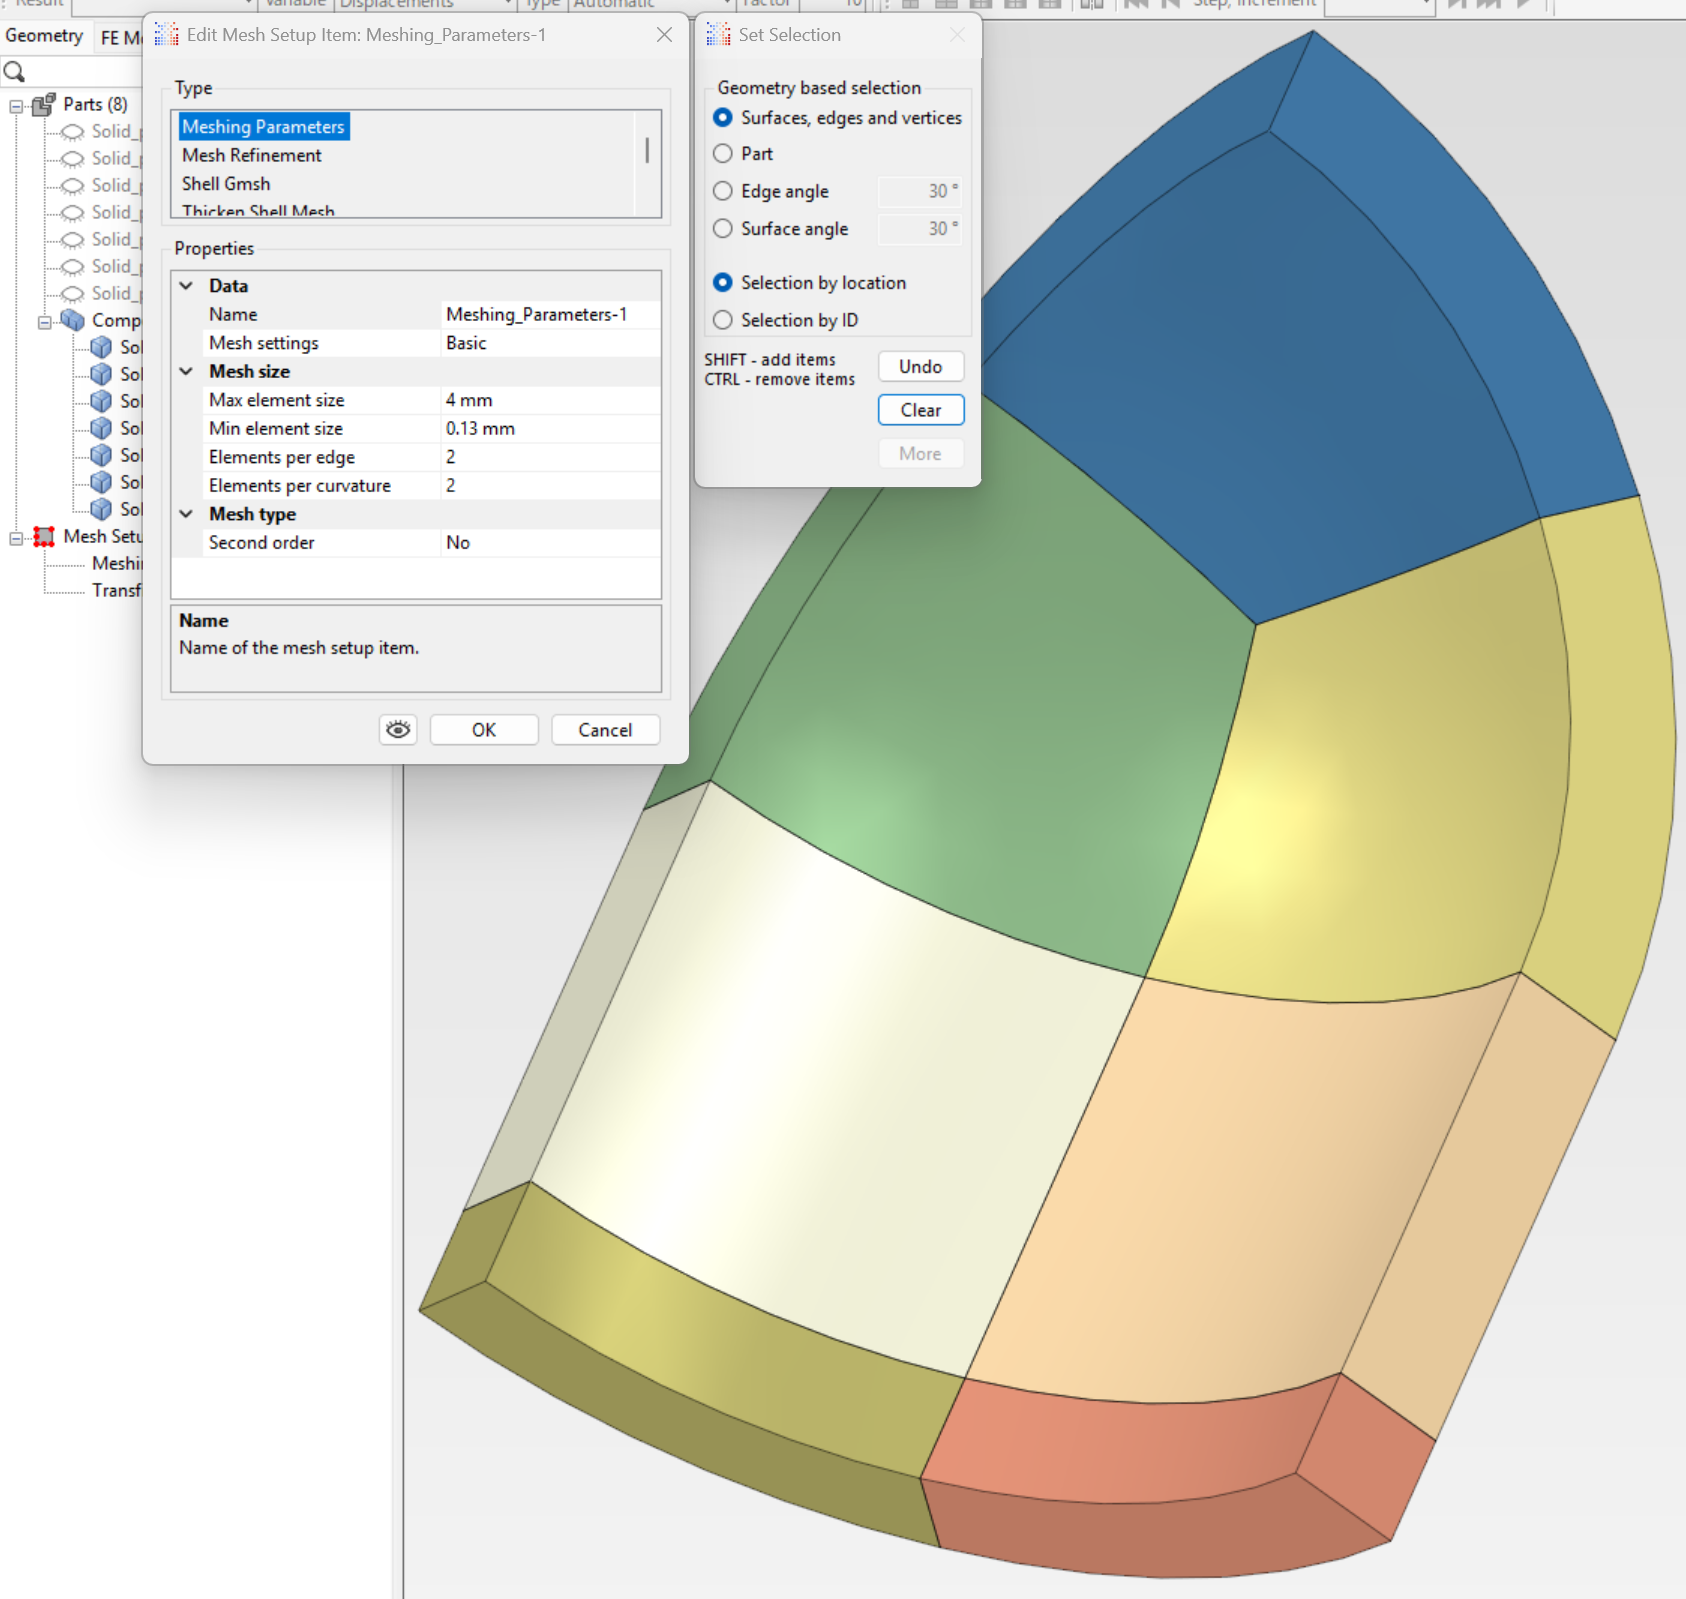
\includegraphics[keepaspectratio,scale=0.30]{images/sc7.png}}
            \only<3>{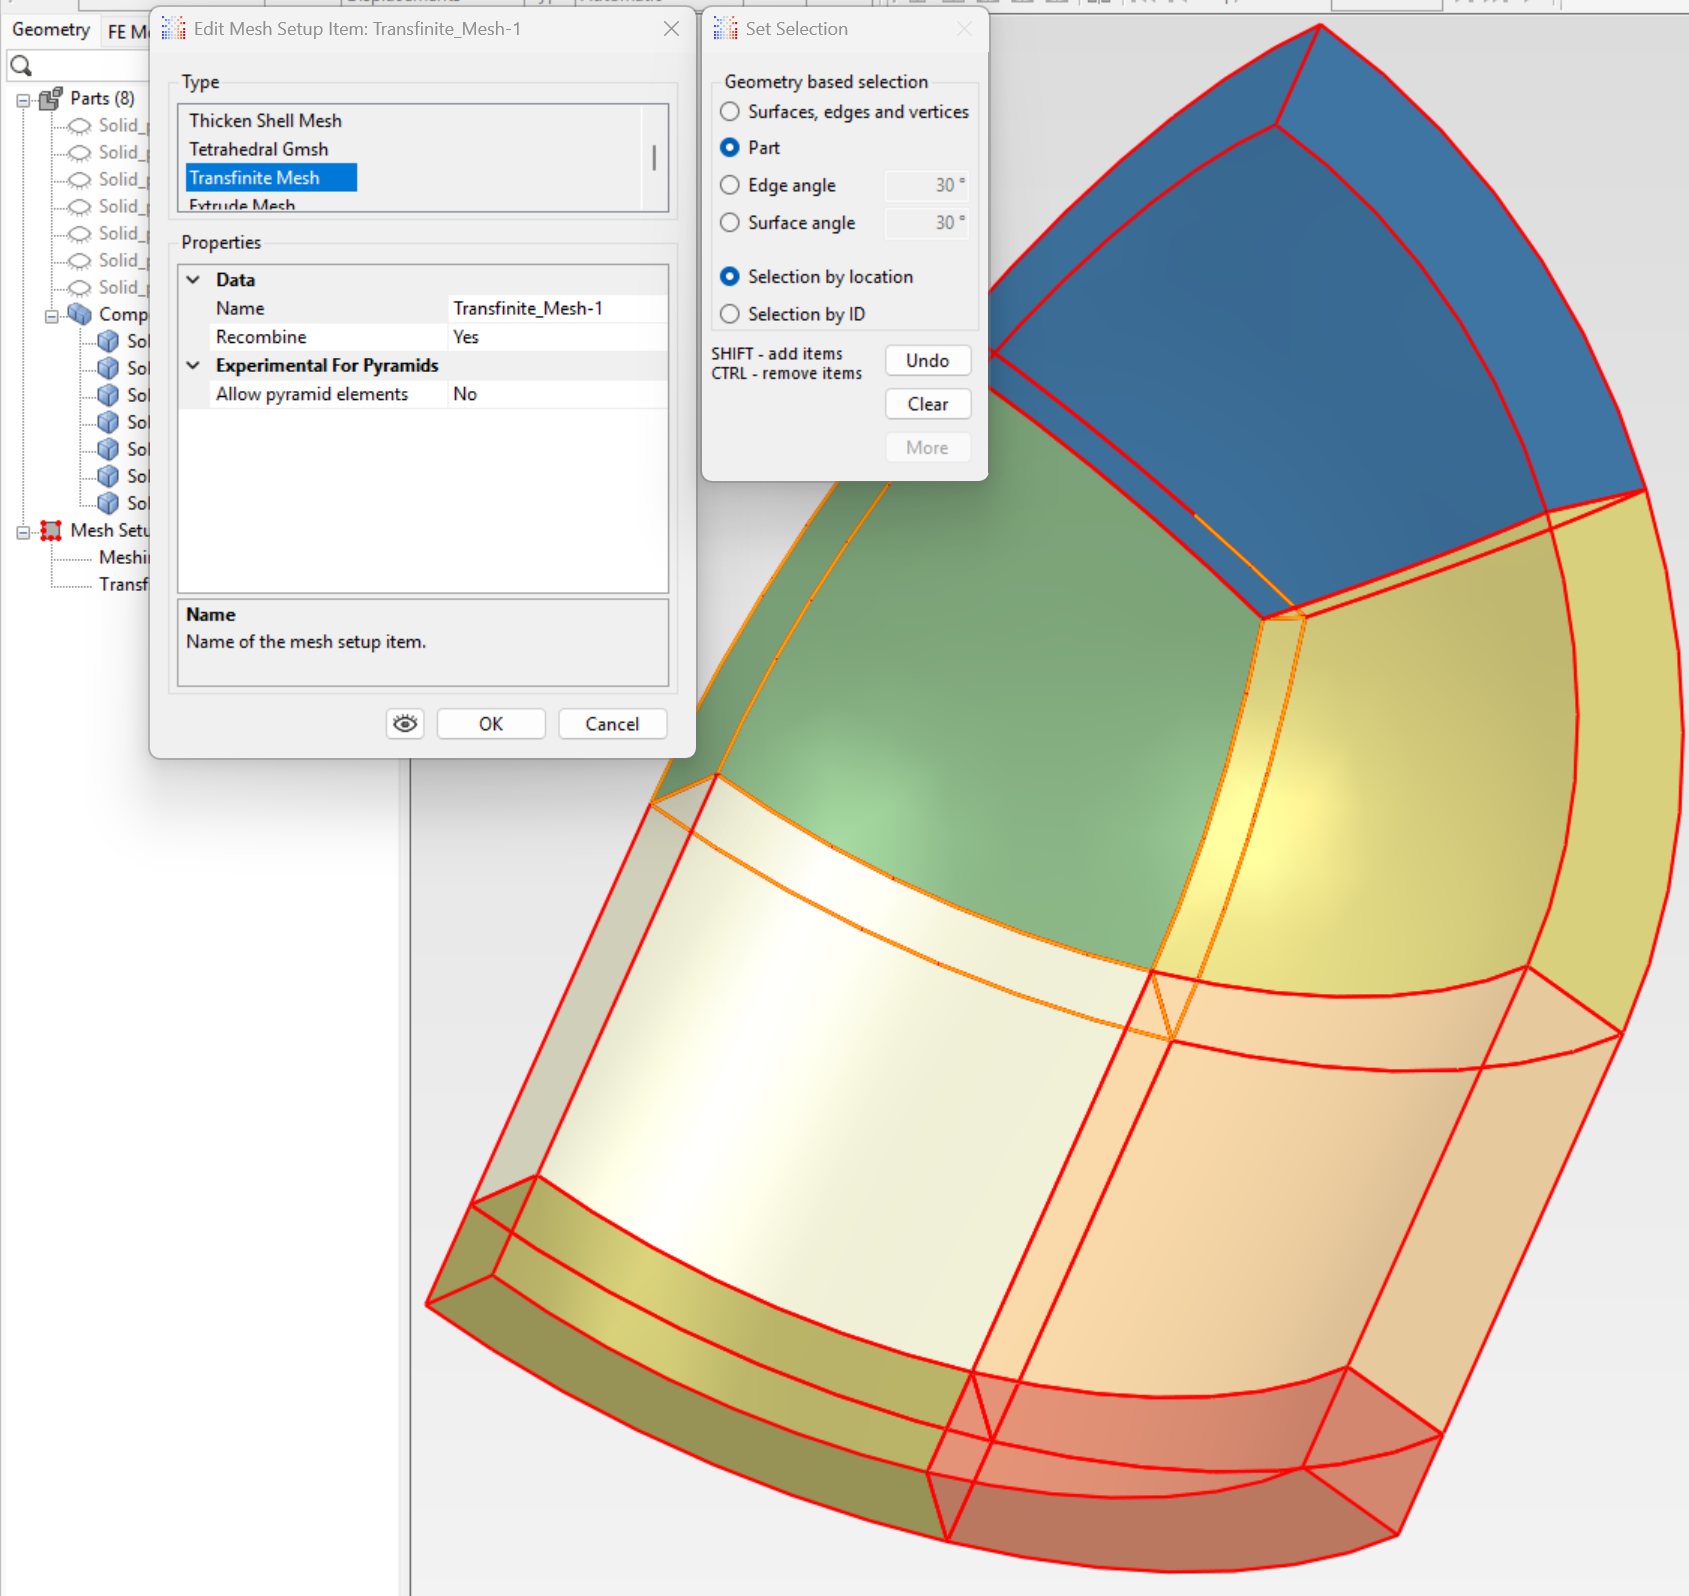
\includegraphics[keepaspectratio,scale=0.30]{images/sc8.png}}
            \only<4->{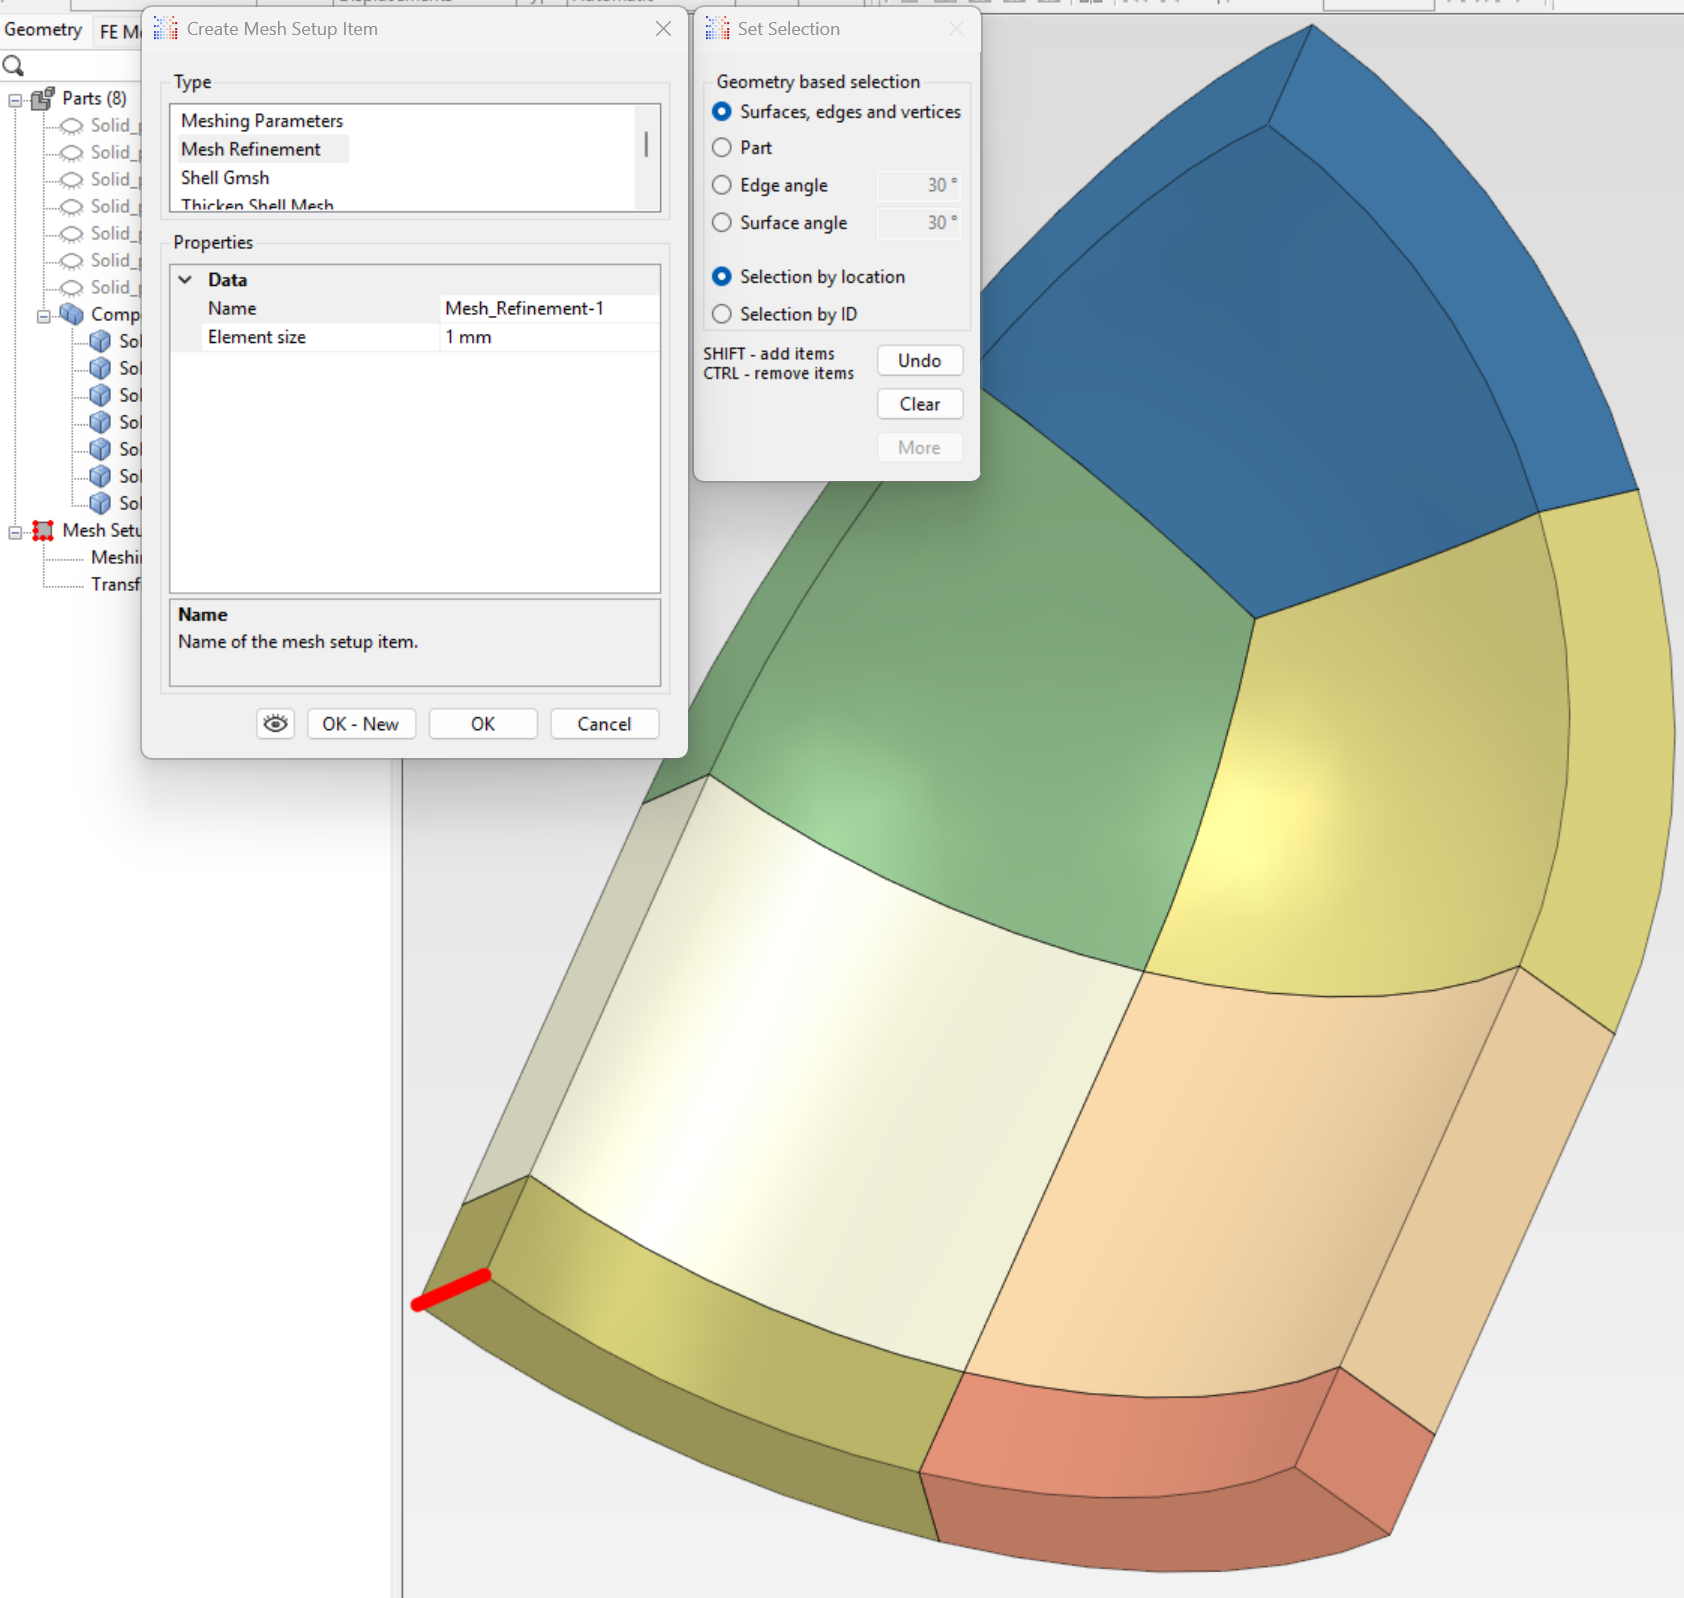
\includegraphics[keepaspectratio,scale=0.30]{images/sc9.png}}
            \caption{メッシュ設定の概要}
          \end{overlayarea}
        \end{center}
      \end{figure}
    \end{column}
  \end{columns}
  \only<1>{
    \begin{textblock*}{160pt}(200pt,73pt)
      \begin{tikzpicture}
         \node[rectangle,fill=cud_yellow,text width=90pt,text centered,rounded corners,minimum height=40pt](s) at (1cm,1cm) { \scriptsize 全体のメッシュ\\サイズを4mmに設定};
         \draw[->, draw=cud_red, line width=1pt] (10pt,50pt) -- (80pt,100pt);
      \end{tikzpicture}
    \end{textblock*}
  }
  \only<2>{
    \begin{textblock*}{160pt}(200pt,90pt)
      \begin{tikzpicture}
         \node[rectangle,fill=cud_yellow,text width=90pt,text centered,rounded corners,minimum height=40pt](s) at (1cm,1cm) { \scriptsize Second Order\\は No};
         \draw[->, draw=cud_red, line width=1pt] (10pt,50pt) -- (80pt,76pt);
      \end{tikzpicture}
    \end{textblock*}
  }
  \only<4>{
    \begin{textblock*}{100pt}(248pt,65pt)
      \begin{tikzpicture}
	      \node[rectangle,fill=cud_yellow,text width=70pt,text centered,rounded corners,minimum height=40pt](s) at (1cm,1cm) { \scriptsize この線を\\1mm(20分割)};
         \draw[->, draw=cud_red, line width=1pt] (20pt,50pt) -- (40pt,180pt);
         \draw[->, draw=cud_red, line width=1pt] (20pt,50pt) -- (37pt,70pt);
      \end{tikzpicture}
    \end{textblock*}
  }
\end{frame}
